 %\documentclass[aspectratio=43]{beamer} %For normal presentation (comment otherwise)
\documentclass[aspectratio=169]{beamer} %for widescreen presentation
\usetheme{Marburg}
\usefonttheme{serif}\usepackage{ulem}
\usecolortheme{default}%albatross, crane, beetle, dove, fly, seagull, wolverine e beaver.
\setbeamertemplate{frametitle}[default][center]
%%%%%%%%%%%%%%%%%%%%%%%%%%%%%%%%%%%%%%%%%%%%%%%%%%%%%%%%%%%%%%%%%%%%%%%%%%%%%%%%%%%%%%%%%%%%%%%
%%%%%%%%%%%%%%%%%%%%%%%%%%%%%%%%%%%%%%EXTRA PACTAGES%%%%%%%%%%%%%%%%%%%%%%%%%%%%%%%%%%%%%%%%%%%
\usepackage[utf8]{inputenc}
\usepackage[T1]{fontenc}
\usepackage[scaled]{helvet}
\renewcommand*\familydefault{\sfdefault}
\usepackage[portuguese, english]{babel}
\usepackage[round]{natbib}
\usepackage{hyperref} 
\usepackage{tcolorbox}
\usepackage{graphicx} % Required for including images
\usepackage{graphics}
%\usepackage[dvips]{graphicx} 
\graphicspath{{images/}} % Location of the graphics files
\usepackage{booktabs} % Top and bottom rules for table
\usepackage[font=small,labelfont=bf]{caption}%specifies captions on tables and figures
\usepackage{amsfonts, amsmath, amsthm, amssymb} % For math fonts, symbols and environments
\usepackage{wrapfig} % Allows wrapping text around tables and figures
\usepackage{makeidx}
\usepackage{epstopdf}%adiciona imagens em formato eps no pdf.
\usepackage{subfigure}%cria ambientes de multifiguras
\usepackage{float}%coloca as figuras exatamente aonde você quer
\usepackage{times}
\usepackage{tikz}%pacote para fazer fluxogramas
\usepackage{verbatim}%
\usepackage{multicol}
\usepackage{xcolor}
\usepackage[makeroom]{cancel}
\usepackage[framemethod=tikz]{mdframed}
\usepackage{hyperref} 
\usepackage{smartdiagram}
%\smartdiagramset{uniform color list=gray!60!black for 6 items,
%back arrow disabled=false}
\usepackage{booktabs} % Top and bottom rules for table
\usepackage[font=small,labelfont=bf]{caption} % Required for specifying captions to
\usepackage{cancel} 
\usepackage{multicol}

%%%%%%%%%%%%%%%%%%%%%%%%%%%%% PREAMBLE %%%%%%%%%%%%%%%%%%%%%%%%%%
%\subtitle{}
\author[Carreira et. al]{Carreira,V.R.$^{1}$;  Venancio,I.M.$^{1}$; Belem,A.L.$^{1}$; Nascimento,R.A.$^{1}$; Affonso,P.V.A.$^{1}$; Viegas,I.A.F.S.$^{2}$; Spigolon,A.L.D.$^{2}$;  Albuquerque,A.L.S.$^{1}$} 
\title{Stochastic TOC modeling for East African Rift System Lakes, a possible pre-salt analogous}
%\subtitle{\color{black}{Carreira,V.R. and  Venancio,I.M. and Belem,A.L. and Nascimento,R.A. and Affonso,P.V.A. and Viegas,I.A.F.S., Spigolon,A.L.D.,  Albuquerque,A.L.S.}}
\institute{$1$ Federal Fluminense University - UFF (in Portuguese) \\
$2$ PETROBRAS}
\date{August 11, 2023}
%\subject{Grupo de Pesquisa em Ambientes Lacustres}
\setbeamertemplate{footline}[frame number]
%\setbeamercovered{transparent}
\setbeamertemplate{navigation symbols}{}
% Tela cheia
\hypersetup{pdfpagemode=FullScreen}
\usepackage{ragged2e}
%\justifying
%\addtobeamertemplate{headline}{} 

%%%%%%%%%%%%%%%%%%%%%%%%%%%%% PRESENTATION %%%%%%%%%%%%%%%%%%%%%%%%%%%%%%%
\begin{document}
\bgroup
\makeatletter
\setbeamertemplate{footline}
\makeatother
\egroup
\scriptsize 
\addtobeamertemplate{navigation symbols}{}{\hskip6pt\raisebox{2pt}{\color{blue}\insertframenumber}}
\setcounter{framenumber}{0}



{
\usebackgroundtemplate{
\centering
\includegraphics[width=\paperwidth,height=\paperheight]{images/fundo.jpg}
}
\begin{frame}
\maketitle
	
\end{frame}
}



%%% DEFININDO O PROBLEMA
\section{Problem set}


{
\usebackgroundtemplate{
\centering
\includegraphics[width=\paperwidth,
height=\paperheight]{images/fundopreto.jpg}
}
{
\begin{frame}
	\vspace{1cm}
	\begin{large}
		\begin{center}
	          \color{orange}{... somewhere in the ancient earth  ...}
		\end{center}
	\end{large}
\pause
	\begin{figure}
	\includegraphics[scale=0.27]{images/150ma.png}
	\end{figure}
\color{yellow}{~150 My ago}
\end{frame}
}
}

{
\usebackgroundtemplate{
\centering
\includegraphics[width=\paperwidth,
height=\paperheight]{images/fundopreto.jpg}
}
{
\begin{frame}
	\vspace{1cm}
	\begin{large}
		\begin{center}
	          \color{orange}{... somewhere in the ancient earth  ...}
		\end{center}
	\end{large}

	\begin{figure}
	\includegraphics[scale=0.27]{images/120ma.png}
	\end{figure}
\color{yellow}{~120 My ago}
\end{frame}
}
}

{
\usebackgroundtemplate{
\centering
\includegraphics[width=\paperwidth,
height=\paperheight]{images/fundo.jpg}
}
{
\begin{frame}
	\vspace{1cm}
	\begin{figure}
	\includegraphics[scale=0.3]{images/aptianoT.png}
		\caption{143My ago, lakes were formed. \citep{Scotese2013} }
	\end{figure}
\end{frame}
}
}


{
\usebackgroundtemplate{
\centering
\includegraphics[width=\paperwidth,
height=\paperheight]{images/fundo.jpg}
}
{
\begin{frame}
%\frametitle{\textcolor{blue}{Function lake}}

	\begin{figure}
		\centering
		\includegraphics[scale=0.4]{images/HL.png}
	\end{figure}
	\pause
\begin{equation}
	\begin{huge}
         TOC = f(\alpha,\gamma,\delta,...)  \nonumber
	\end{huge}
\end{equation}
\end{frame}
}
}

{
\usebackgroundtemplate{
\centering
\includegraphics[width=\paperwidth,
height=\paperheight]{images/fundo.jpg}
}
{
\begin{frame}
%\frametitle{\textcolor{blue}{Function lake}}
	\vspace{0.1cm}
	\begin{figure}
		\centering
		\includegraphics[scale=0.4]{images/HL.png}
	\end{figure}
\begin{equation}
	TOC = \cancelto{unknow}{f(\alpha,\gamma,\delta,...)}  \nonumber
\end{equation}
\end{frame}
}
}






{
\usebackgroundtemplate{
\centering
\includegraphics[width=\paperwidth,
height=\paperheight]{images/fundopreto.jpg}
}
{
\begin{frame}
	\vspace{1cm}
	\begin{large}
		\begin{center}
			\color{orange}{Modern Analogous}
		\end{center}
	\end{large}
\pause
	\begin{figure}
	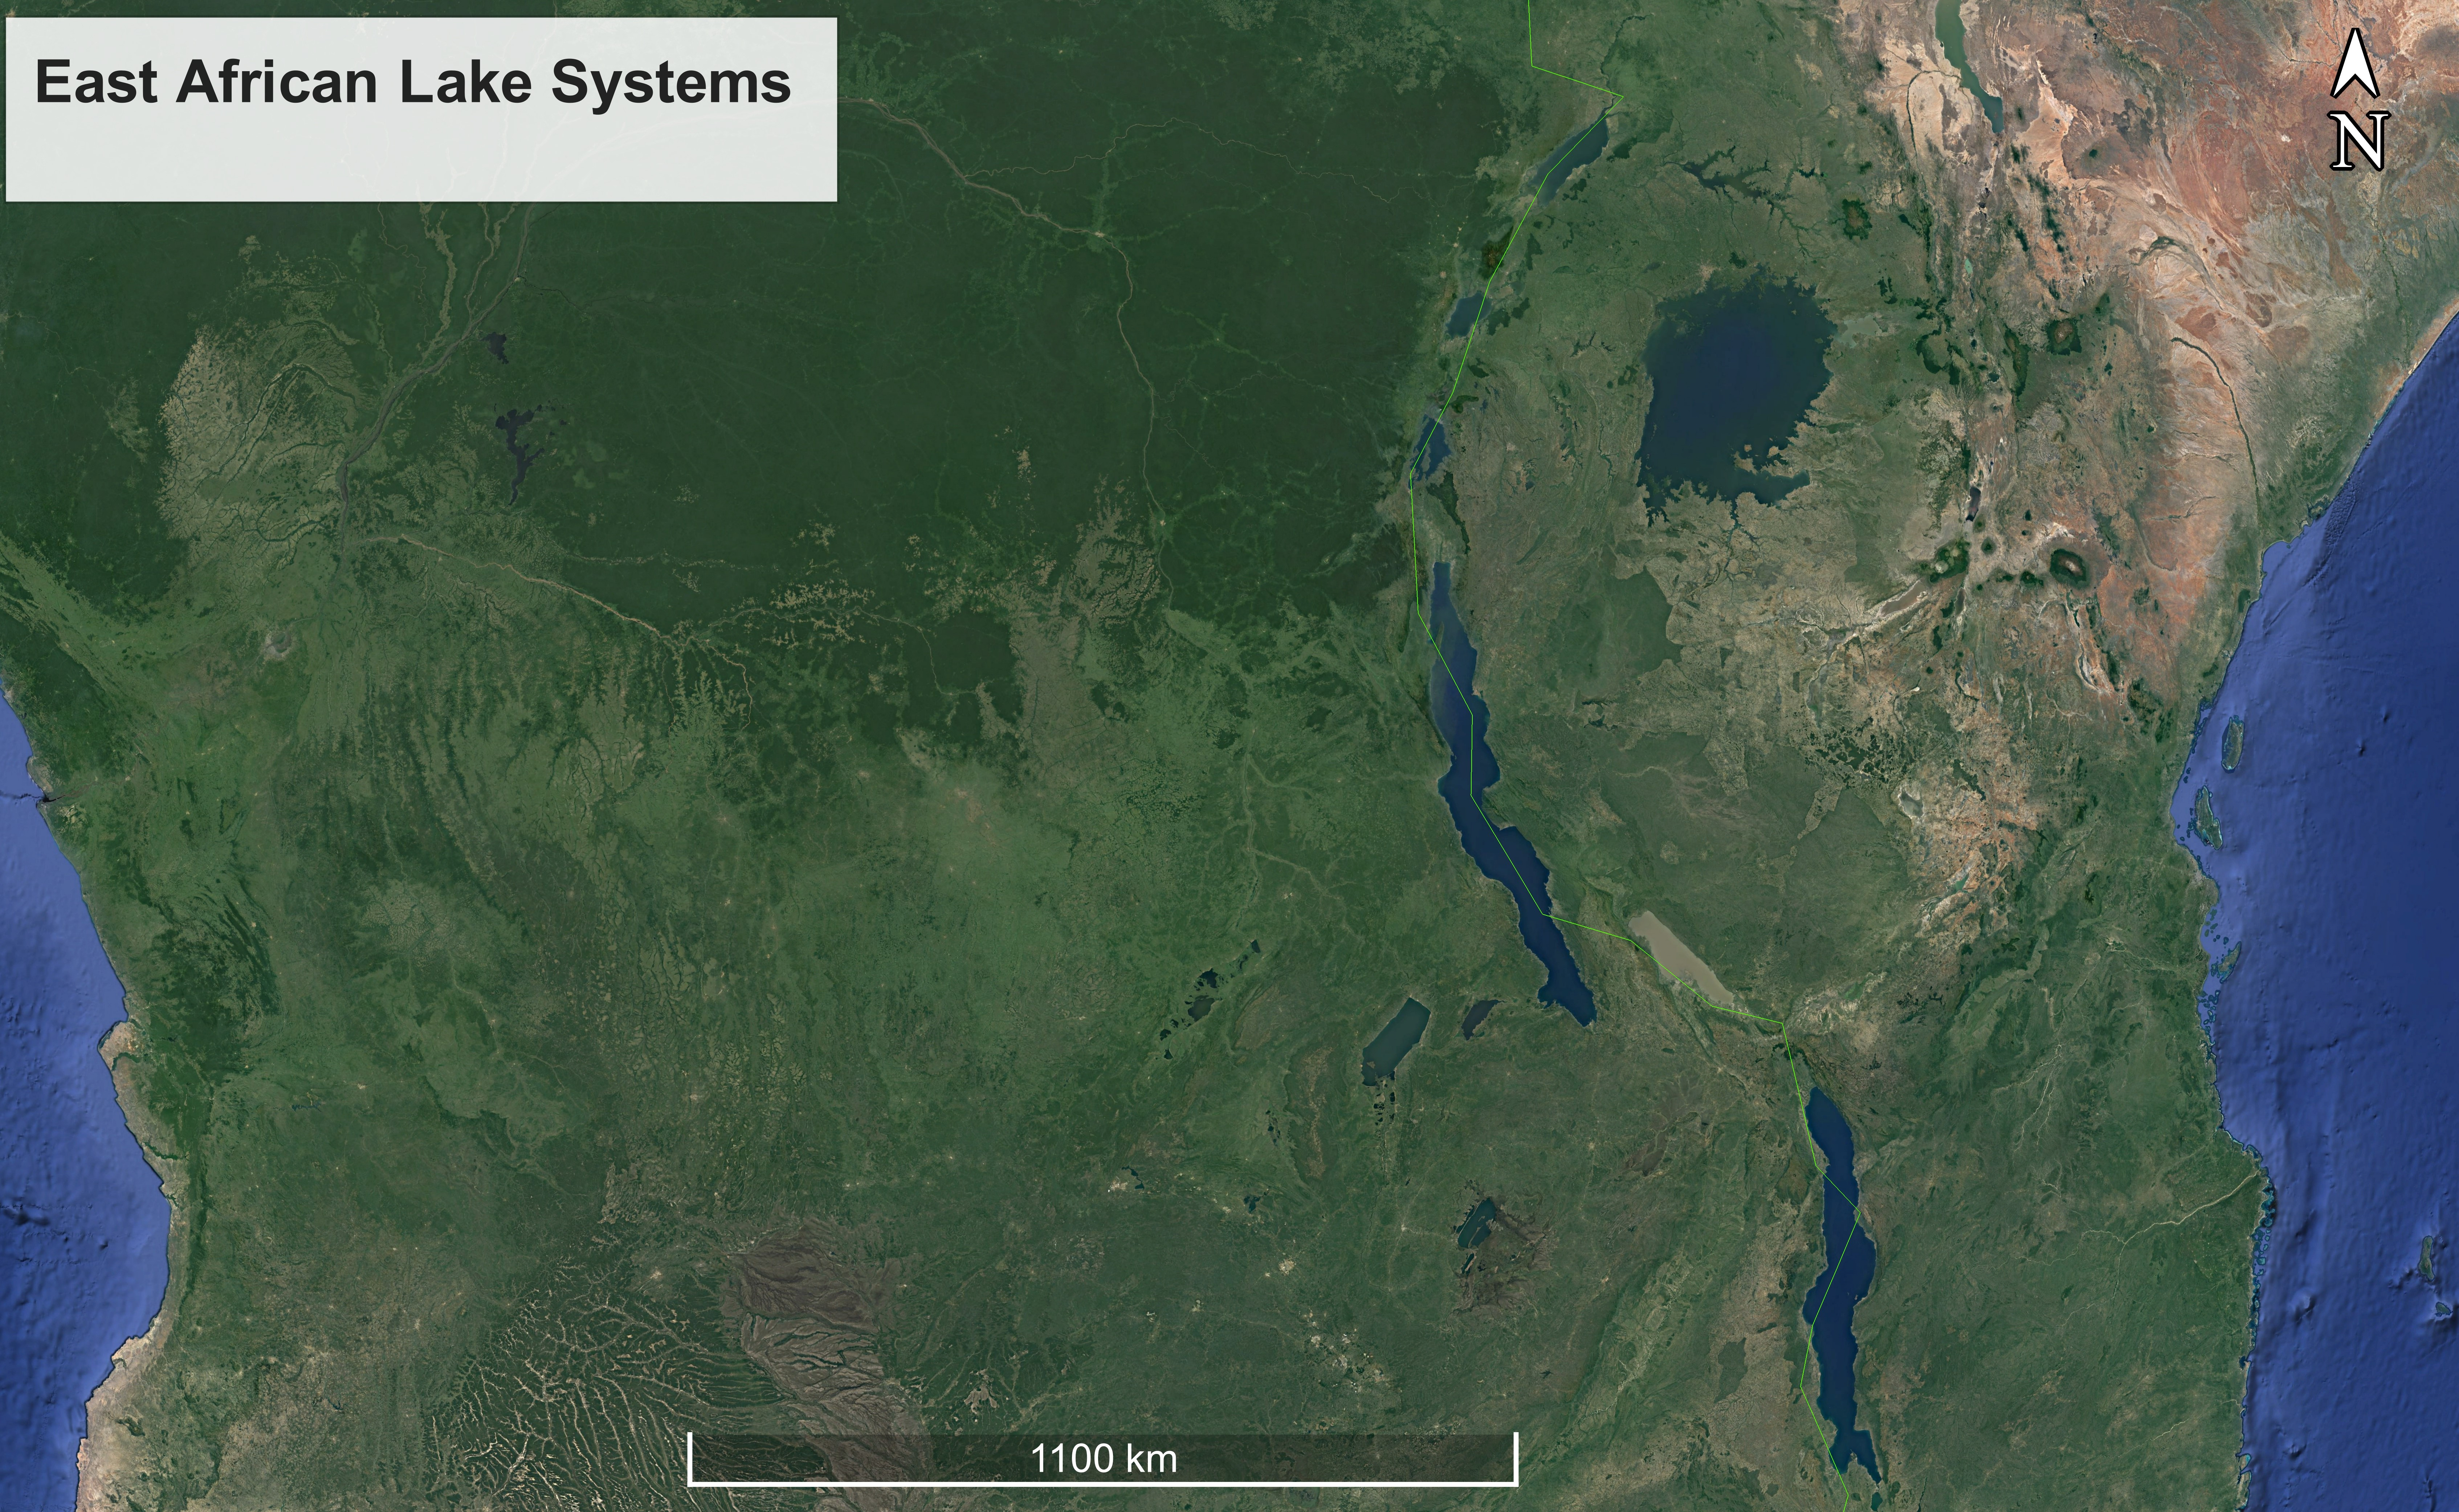
\includegraphics[scale=0.05]{images/ALS.jpg}
	\end{figure}
	\pause
	
\color{yellow}{Considering an initial Rift perspective}
\end{frame}
}
}



%%% MOSTRAR OS OBJETIVOS DO TRABALHO
\section{Objectives}

{
\usebackgroundtemplate{
\centering
\includegraphics[width=\paperwidth,
height=\paperheight]{images/fundo.jpg}
}

{ \begin{frame}
	\vspace{1cm}
	\begin{center}
	\begin{large}
	\color{blue}{Objectives}
	\end{large}
	\end{center}
\begin{flushright}
    \begin{columns}

    \column{0.6\textwidth}
        \centering
	     	\begin{figure}
		\centering
		\includegraphics[scale=0.3]{images/HL.png}
	\end{figure}
    \column{0.4\textwidth}
        \centering
         \begin{itemize}
          \item Define the main variables that interact in actual lakes;   
          \pause
           \item Such lakes should be a pre-salt analogous;
           \pause
          \item Predictive TOC model for lakes;
           \pause
           \item Create and publicize a data table used to mimetic TOC in real lake systems;
           \pause
           \item Define the best membership function for the studied lakes.
     
         \end{itemize}
    \end{columns}

\end{flushright}


\end{frame} }



% INTRODUCAO
\section{Introduction}

{
\usebackgroundtemplate{
\centering
\includegraphics[width=\paperwidth,
height=\paperheight]{images/fundo.jpg}
}

{ \begin{frame}
	\vspace{1cm}
	\begin{center}
	\begin{large}
	\color{blue}{Pre-salt lakes}
	\end{large}
	\end{center}
\begin{flushright}
    \begin{columns}
   \column{0.6\textwidth}
        \centering
         \begin{figure}
		\centering
		\includegraphics[scale=0.23]{images/aptianoT.png}
	\end{figure}

    \column{0.3\textwidth}
        \centering
         \begin{itemize}
          \item This distinctive set of lakes existed throughout the Lower Cretaceous    
          \pause
           \item It has a wide distribution and its record includes the sedimentary basins of the eastern margin as well as the sedimentary basins of the equatorial margin
           \pause
          \item The record of large layers of salt is not decisive for the existence of these lakes.
           \pause
     
         \end{itemize}	     	
    \end{columns}

\end{flushright}

\begin{flushright}
\citep{kelts1988,Talbot1988,Goncalves2001,Wright2018,Boyd2015,Neves2019}
\end{flushright}
\end{frame} }

{
\usebackgroundtemplate{
\centering
\includegraphics[width=\paperwidth,
height=\paperheight]{images/fundo.jpg}
}

{ \begin{frame}
	\vspace{1cm}
	\begin{center}
	\begin{large}
	\color{blue}{Pre-salt lakes}
	\end{large}
	\end{center}
\begin{flushright}
    \begin{columns}

    \column{0.6\textwidth}
        \centering
         \begin{figure}
		\centering
		\includegraphics[scale=0.38]{images/relacaoPE.png}
	\end{figure}


    \column{0.3\textwidth}
        \centering
         \begin{itemize}
          \item The relation precipitation/evaporation induces the preservation factor;     
          \pause
           \item The sedimentation rate, distance of the source area, and the depths of the lake have a direct impact on the preservation factor;
           \pause
          \item Factors such as pH, dissolved oxygen, and primary productivity warrant consideration.
          
     
         \end{itemize}	     	

    \end{columns}

\end{flushright}

\begin{flushright}
\citep{kelts1988,Talbot1988,Goncalves2001,Wright2018,Boyd2015,Neves2019}
\end{flushright}
\end{frame} }



{
\usebackgroundtemplate{
\centering
\includegraphics[width=\paperwidth,
height=\paperheight]{images/fundo.jpg}
}

{ \begin{frame}
	\vspace{1cm}
	\begin{center}
	\begin{large}
	\color{blue}{Fuzzy system}
	\end{large}
	\end{center}
\begin{flushright}
    \begin{columns}

    \column{0.6\textwidth}
        \centering
         \begin{figure}
		\centering
		\includegraphics[scale=0.4]{images/fuzzy_logic.png}
	\end{figure}


    \column{0.3\textwidth}
        \centering
         \begin{itemize}
          \item Fuzzy sets are defined by an interval within a linguistic variable 
          \pause
          \item Linguistic variables are known as antecedents or consequents depending on the inputs or outputs of the model    
          \pause
           \item These ranges are defined within the linguistic terms
           \pause
          \item Each linguistic term is related to each other through a membership function
           \pause
           \item There is no formal basis for determining which is the best membership function for each linguistic variable.
           \pause
     
         \end{itemize}	     	

    \end{columns}

\end{flushright}

\begin{flushright}
\citep{Jafelice2012,josh2019,Siddig2021}
\end{flushright}
\end{frame} }







% METODOLOGIA
\section{Methodology}

{
\usebackgroundtemplate{
\centering
\includegraphics[width=\paperwidth,
height=\paperheight]{images/fundo.jpg}
}

{ \begin{frame}
	\vspace{1cm}
	\begin{center}
	\begin{large}
	\color{blue}{Methodological flowchart}
	\end{large}
	\end{center}


    \begin{columns}

    \column{0.5\textwidth}
        \centering
      \begin{figure}
		\centering
		\includegraphics[scale=0.6]{images/methodology.png}
	\end{figure}
	     	\pause
    \column{0.5\textwidth}
        \centering
\begin{small}
\begin{equation}
RMS = \sqrt{\frac{1}{n}\sum_{i=1}^{n}(x_i - \hat{x_i})^2} \nonumber
\end{equation}
\end{small}
    \end{columns}








\end{frame} }


{
\usebackgroundtemplate{
\centering
\includegraphics[width=\paperwidth,
height=\paperheight]{images/fundo.jpg}
}
{
\begin{frame}
	\footnotesize
	\begin{table}
		\caption{ East African Lakes Database. In red is TOC, defined as the model consequent variable. \citep{Talbot1988,Bronikowska2021,ZSWZIA2016}} % title 
		\centering
		\begin{tabular}{c| c c c c c c c c c} 
			\hline\hline %inserts double horizontal lines
			Lake & \color{red}{TOC} & AD & MD & pH &$ O_{2}$ & SR & GRA & SEL & PP \\ [0.5ex] %heading 
			\hline % inserts single horizontal line
			Edward    & \color{red}{11.62} & 17 & 112 & 9.10 & 2.50 & 2.8  & 0.06 & 1    & 43.30 \\ 
			Motubu    & \color{red}{2.81}  & 70 & 85  & 8.90 & 0.02 & 0.9  & 0.2  & 25   & 600   \\
			Kivu      & \color{red}{7.14}  & 240& 480 & 8.60 & 11.76& 8.00 & 0.10 & 0.02 & 264   \\
			Tanganyika& \color{red}{4.81}  & 572& 1470& 8.30 & 9.16 & 1.00 & 0.002& 0.02 &1.40   \\
			Victoria  & \color{red}{11.23} & 40 & 80  & 9.30 & 0.12 & 0.82 & 0.002& 0.02 &6.25   \\[1ex] % [1ex] adds vertical space
			\hline %inserts single line
		\end{tabular}
		\label{lakesdatabase} % is used to refer this table in the text
	\end{table} 
      where TOC is Total Organic Carbon in $\%$, AD is average depth in $m$, MD is maximum depth in $m$,  SR is sedimentation rate $(cm/kyear)$, GRA is grain size deposit in $mm$, SEL grain selection in $mm$, PP is primary productivity in  $(gC/m^{2}/year)$.  

\end{frame}
}
}




% RESULTADOS E DISCUSSOES
\section{Results and Discussion}


{
\usebackgroundtemplate{
\centering
\includegraphics[width=\paperwidth,
height=\paperheight]{images/fundo.jpg}
}

{ \begin{frame}
	\vspace{1cm}
	\begin{center}
	\begin{large}
	\color{blue}{Victoria Lake}
	\end{large}
	\end{center}
	    \begin{figure}
		\centering
		\includegraphics[scale=0.45]{images/COT_variables.png}
	\end{figure}
	\pause
\begin{flushright}
    \begin{columns}

    \column{0.5\textwidth}
        \centering
         \begin{figure}
		\centering
		\includegraphics[scale=0.4]{images/COT_Victoria_triangular.png}
	\end{figure}
	     	
    \column{0.5\textwidth}
        \centering
         \begin{figure}
		\centering
		\includegraphics[scale=0.4]{images/COT_Victoria_trapezoidal.png}
	\end{figure}
    \end{columns}

\end{flushright}

\end{frame} }


{
\usebackgroundtemplate{
\centering
\includegraphics[width=\paperwidth,
height=\paperheight]{images/fundo.jpg}
}

{ \begin{frame}
	\vspace{1cm}
	\begin{center}
	\begin{large}
	\color{blue}{Tanganyika Lake}
	\end{large}
	\end{center}
	    \begin{figure}
		\centering
		\includegraphics[scale=0.45]{images/COT_variables.png}
	\end{figure}
		
	
\begin{flushright}
    \begin{columns}

    \column{0.5\textwidth}
        \centering
         \begin{figure}
		\centering
		\includegraphics[scale=0.4]{images/COT_Tanganyika_triangular.png}
	\end{figure}
	     	
    \column{0.5\textwidth}
        \centering
         \begin{figure}
		\centering
		\includegraphics[scale=0.4]{images/COT_Tanganyika_trapezoidal.png}
	\end{figure}
    \end{columns}

\end{flushright}

\end{frame} }




{
\usebackgroundtemplate{
\centering
\includegraphics[width=\paperwidth,
height=\paperheight]{images/fundo.jpg}
}

{ \begin{frame}
	\vspace{1cm}
	\begin{center}
	\begin{large}
	\color{blue}{Kivu Lake}
	\end{large}
	\end{center}
	    \begin{figure}
		\centering
		\includegraphics[scale=0.45]{images/COT_variables.png}
	\end{figure}
		
	
	
\begin{flushright}
    \begin{columns}

    \column{0.5\textwidth}
        \centering
         \begin{figure}
		\centering
		\includegraphics[scale=0.4]{images/COT_Kivu_triangular.png}
	\end{figure}
	     	
    \column{0.5\textwidth}
        \centering
         \begin{figure}
		\centering
		\includegraphics[scale=0.4]{images/COT_Kivu_trapezoidal.png}
	\end{figure}
    \end{columns}

\end{flushright}

\end{frame} }


{
\usebackgroundtemplate{
\centering
\includegraphics[width=\paperwidth,
height=\paperheight]{images/fundo.jpg}
}

{ \begin{frame}
	\vspace{1cm}
	\begin{center}
	\begin{large}
	\color{blue}{Edward Lake}
	\end{large}
	\end{center}
	    \begin{figure}
		\centering
		\includegraphics[scale=0.45]{images/COT_variables.png}
	\end{figure}
		
	
	
\begin{flushright}
    \begin{columns}

    \column{0.5\textwidth}
        \centering
         \begin{figure}
		\centering
		\includegraphics[scale=0.4]{images/COT_Edward_triangular.png}
	\end{figure}
	     	
    \column{0.5\textwidth}
        \centering
         \begin{figure}
		\centering
		\includegraphics[scale=0.4]{images/COT_Edward_trapezoidal.png}
	\end{figure}
    \end{columns}

\end{flushright}

\end{frame} }

{
\usebackgroundtemplate{
\centering
\includegraphics[width=\paperwidth,
height=\paperheight]{images/fundo.jpg}
}

{ \begin{frame}
	\vspace{1cm}
	\begin{center}
	\begin{large}
	\color{blue}{Motubu Lake}
	\end{large}
	\end{center}
	    \begin{figure}
		\centering
		\includegraphics[scale=0.45]{images/COT_variables.png}
	\end{figure}
		
	
	
\begin{flushright}
    \begin{columns}

    \column{0.5\textwidth}
        \centering
         \begin{figure}
		\centering
		\includegraphics[scale=0.4]{images/COT_Motubu_triangular.png}
	\end{figure}
	     	
    \column{0.5\textwidth}
        \centering
         \begin{figure}
		\centering
		\includegraphics[scale=0.4]{images/COT_Motubu_trapezoidal.png}
	\end{figure}
    \end{columns}

\end{flushright}

\end{frame} }






{
\usebackgroundtemplate{
\centering
\includegraphics[width=\paperwidth,
height=\paperheight]{images/fundo.jpg}
}
{
\begin{frame}
	\footnotesize
	\begin{table}
		\caption{Results} % title 
		\centering
		\begin{tabular}{c| c| c c c} 
			\hline\hline %inserts double horizontal lines
			Lake & membership & $TOC_{obs} (\%)$ & $TOC_{calc} (\%)$ & RMS $(\%)$\\ [0.5ex] %heading 
			\hline % inserts single horizontal line
			Edward & triangular & 11.62 & 13.95  & 2.33  \\ 
			Motubu & triangular & 2.81  & 5.89   & 3.07  \\
			Kivu   & triangular & 7.14  & 7.67   & 0.53  \\
		Tanganyika & triangular & 4.81  & 4.67   & 0.13  \\
		Victoria   & triangular & 11.23 & 10.87  & 0.36  \\
		\hline
		    Edward & trapezoidal & 11.62 & 15.24  & 3.62  \\ 
			Motubu & trapezoidal & 2.81  & 5.15   & 2.34  \\
			Kivu   & trapezoidal & 7.14  & 10.72  & 3.58  \\
		Tanganyika & trapezoidal & 4.81  & 4.79   & 0.01  \\
		Victoria   & trapezoidal & 11.23 & 10.14  & 1.08  \\[1ex] % [1ex] adds vertical space
			\hline %inserts single line
		\end{tabular}
		\label{lakesdatabase} % is used to refer this table in the text
	\end{table} 


\end{frame}
}
}


% CONCLUSOES 
\section{Conclusion}

{
\usebackgroundtemplate{
\centering
\includegraphics[width=\paperwidth,
height=\paperheight]{images/fundo.jpg}
}

{ \begin{frame}
	\vspace{1cm}
	\begin{center}
	\begin{large}
	\color{blue}{Some conclusions}
	\end{large}
	\end{center}

\begin{itemize}
\item The simulations held for the East African Lake Systems
showed good results for TOC estimation when a lake
TOC function is not known.
\pause
\item  The TOC concentration is
better estimated when triangular membership functions
are applied.
\pause
\item  Results indicates that the organic matter
contents can be estimated considering important
environmental variables such as primary productivity
(maximum of 600 gC/m2/year) and dissolved oxygen, but
also when geological parameters such as sedimentation
rate, granulometry, and selection are considered.
\end{itemize}

\end{frame} }




%%%%%%%%% FINAL %%%%%%%%%%%%%%
\usebackgroundtemplate{
\centering
\includegraphics[width=\paperwidth,height=\paperheight]{images/fundo.jpg}
}
\begin{frame}[allowframebreaks]
	\vspace{1cm}
	\color{blue}{References}
\beamertemplatetextbibitems
\tiny
\bibliographystyle{apalike}
\bibliography{references}
\end{frame}
}
\makeatother

{
\usebackgroundtemplate{
\centering
\includegraphics[width=\paperwidth,height=\paperheight]{images/agradecimento.png}
}	
\begin{frame}
\end{frame}
}


\end{document}
